\documentclass[10pt,twocolumn]{article}

% use the oxycomps style file
\usepackage{oxycomps}

% usage: \fixme[comments describing issue]{text to be fixed}
% define \fixme as not doing anything special
\newcommand{\fixme}[2][]{#2}
% overwrite it so it shows up as red
\renewcommand{\fixme}[2][]{\textcolor{red}{#2}}
% overwrite it again so related text shows as footnotes
%\renewcommand{\fixme}[2][]{\textcolor{red}{#2\footnote{#1}}}

% read references.bib for the bibtex data
\bibliography{references}

% include metadata in the generated pdf file
\pdfinfo{
    /Title (Junior Comprehensive Proposal)
    /Author (Julianne Yotov)
}

% set the title and author information
\title{Junior Comprehensive Proposal}
\author{Julianne Yotov}
\affiliation{Occidental College}
\email{jyotov@oxy.edu}

\begin{document}

\maketitle

\section{Problem Context}

My current comps project is to create a website for beginners to computer programming and coding that offers a variety of coding exercises through which users learn how to effectively test code. My inspiration for this project primarily comes from CodingBat \cite{CodingBat}, a website with coding exercises for both Python and Java. My initial motivation behind this project was largely due to my own experience with taking AP Computer Science in high school. I struggled with many of the coding projects that we were assigned and found that this was largely due to my lack of understanding of basic foundational concepts, such as how to write a proper for loop. When I started doing CodingBat exercises, I found that I enjoyed working through the exercises and gained a lot of confidence in the process. I particularly liked that CodingBat’s pre-written test cases allowed me to easily spot patterns in the cases that were failing, which allowed me to find errors in my code independently. By working on these problems, I was able to put certain skills, such as creating arrays and writing nested loops, into use when working on larger coding projects that involved writing classes with multiple methods.

I was also inspired to pursue a project related to computer science education from my experience remotely tutoring two students in Python, a sixth grade student with some previous experience learning Python, and a high school student with no previous coding experience. From their feedback throughout our sessions, I started to gain a sense of which educational resources were effective. I sometimes started sessions by presenting a new concept, but ensured that they had the opportunity to do a lot of coding practice. Both of them expressed that they enjoyed working through exercises in CodingBat and felt a sense of accomplishment when all of the test cases would pass. However, I found that I struggled to teach them about the importance of testing code outside of CodingBat and did not know how to best present examples. When we worked on writing test cases, whether for a short method or for an entire game we made, I found that my students often didn’t quite know how to best structure their test cases to ensure that they were covering edge cases. 

I began to realize that I myself had never spent a lot of time learning how to properly test my code. It wasn’t until I came to Occidental and took COMP 181 (Advanced Programming) that I actually remember learning about testing, and we had one assignment specifically devoted to testing code, while the importance of it was emphasized throughout the course. I feel that I would have benefited from this level of instruction in high school given how I struggled with coding and understanding my code's errors. This is what ultimately led me to decide to emphasize testing for this project, as this allows me to ensure that I have a specific focus and goal that I would like to achieve. I would like to design my website in such a way that users find the task enjoyable rather than extremely tedious, and that they come to see testing as something that is somewhat similar to editing an essay; it allows you to find issues in your code and fix them. I hope to emphasize the importance of proper testing in a way that ensures that users will be able to take the concepts that they have learned from using my website and apply them to future coding-related projects. I feel that creating this educational website that teaches users how to write test cases for their code can be particularly useful to high school students taking coding classes, undergraduate college students taking introductory computer programming courses, and students taking courses that require coding for a subject area other than computer science. Therefore, this will be the primary audience for my project, and I will be seeking feedback from these groups while creating my website.

\section{Technical Background}

Due to the nature of my project, one of the most important aspects will be deciding how to present information regarding testing and how the website will test the user’s code. Ideally, the user’s test cases won’t be the only cases that are checked; the website will contain some pre-written test cases and generate additional test cases that will be shared with the user, in a similar fashion to CodingBat. Most of the test cases that I have written in the past, as well as all of the pre-written test cases in CodingBat, are unit tests, which typically focus on a specific function or method. Therefore, unit tests are also ideal for my website’s coding exercises. However, it is also important to consider other types of tests. One important software testing technique that I will likely make use of is fuzz testing, which “uses invalid, unexpected, or random data as input and then checks for exceptions such as crashes and potential memory leaks.” There are many advantages to fuzz testing; it helps ensure software security, has the ability to be automated so that many inputs can be tested quickly, and its dynamic nature, allowing it to be used for many different types of inputs \cite{Fuzz}.

A unit test can be converted to a fuzz test. One limitation of unit tests that is fixed by fuzz testing is that “...each input must be added to the test by the developer.” Meanwhile, “one benefit of fuzzing is that it comes up with inputs for your code, and may identify edge cases that the test cases you came up with didn’t reach.” However, unit tests allow for the user to note the expected output of the function or method, since they can control the inputs. On the other hand, fuzz testing does not allow users to do this, as they do not choose the inputs \cite{FuzzTutorial}. Given these differences, I will be sure to consider the potential benefits of fuzz testing and how to utilize fuzz tests to test users’ code. Additionally, fuzz testing will be helpful when I am building my website, as it will help me ensure that it is functioning as intended.  

I will likely be using JavaScript to build my website. In order for this website to function as intended, as outlined in the Methods section, it is essential to consider the different components of web application architecture. The website will likely be a single page application, which “only include[s] the most required elements and information to generate an intuitive and interactive user experience… the content or information is updated on the current page rather than loading a new page from the server for each action performed by the user.” Additionally, “web applications run on the client-side and the server-side.” For the server-side, one “decides the functions of the code on the server and the functions of the code on the browser… [and] also define[s] how these two will function in relation to each other… The server-side code is mainly responsible for creating the page which the user has requested” \cite{Architecture}. I will likely use JavaScript to write this server-side code.  

\section{Prior Work}

As discussed in the Problem Context section, I hope to emulate some of CodingBat’s elements within my project \cite{CodingBat}. As shown in Figure 1, the coding exercises are sorted into groups based on the concepts that they cover, including String, Array (for Java) or List (for Python), Logic (which include logic puzzles). When clicking on an exercise, the instructions are given, below which are listed a few examples of the expected outputs for certain inputs, as shown in Figure 2. The user can then type their code directly into the box below the function or method heading and run their code. Then, a series of test cases will appear, and it is noted whether each output matches the expected output or not, as shown in Figure 3. Finally, once all test cases pass (as in Figure 4), that exercise is marked as completed. CodingBat specifies a certain number of test cases (seven in the coding exercise shown in Figures 2, 3, and 4). While additional test cases are utilized, as demonstrated by the “other tests” row in Figures 3 and 4, the seven tests cover a variety of different cases, such as an empty string and strings with numbers. There are certain incentives to keep users engaged. Completing any three exercises in a section earns the user a star, and earning one star in each section earns the user a 5-star badge, while earning two stars and five stars in each section earns the user a 10-star badge and 25-star badge, respectively.

\begin{figure}
    \centering
    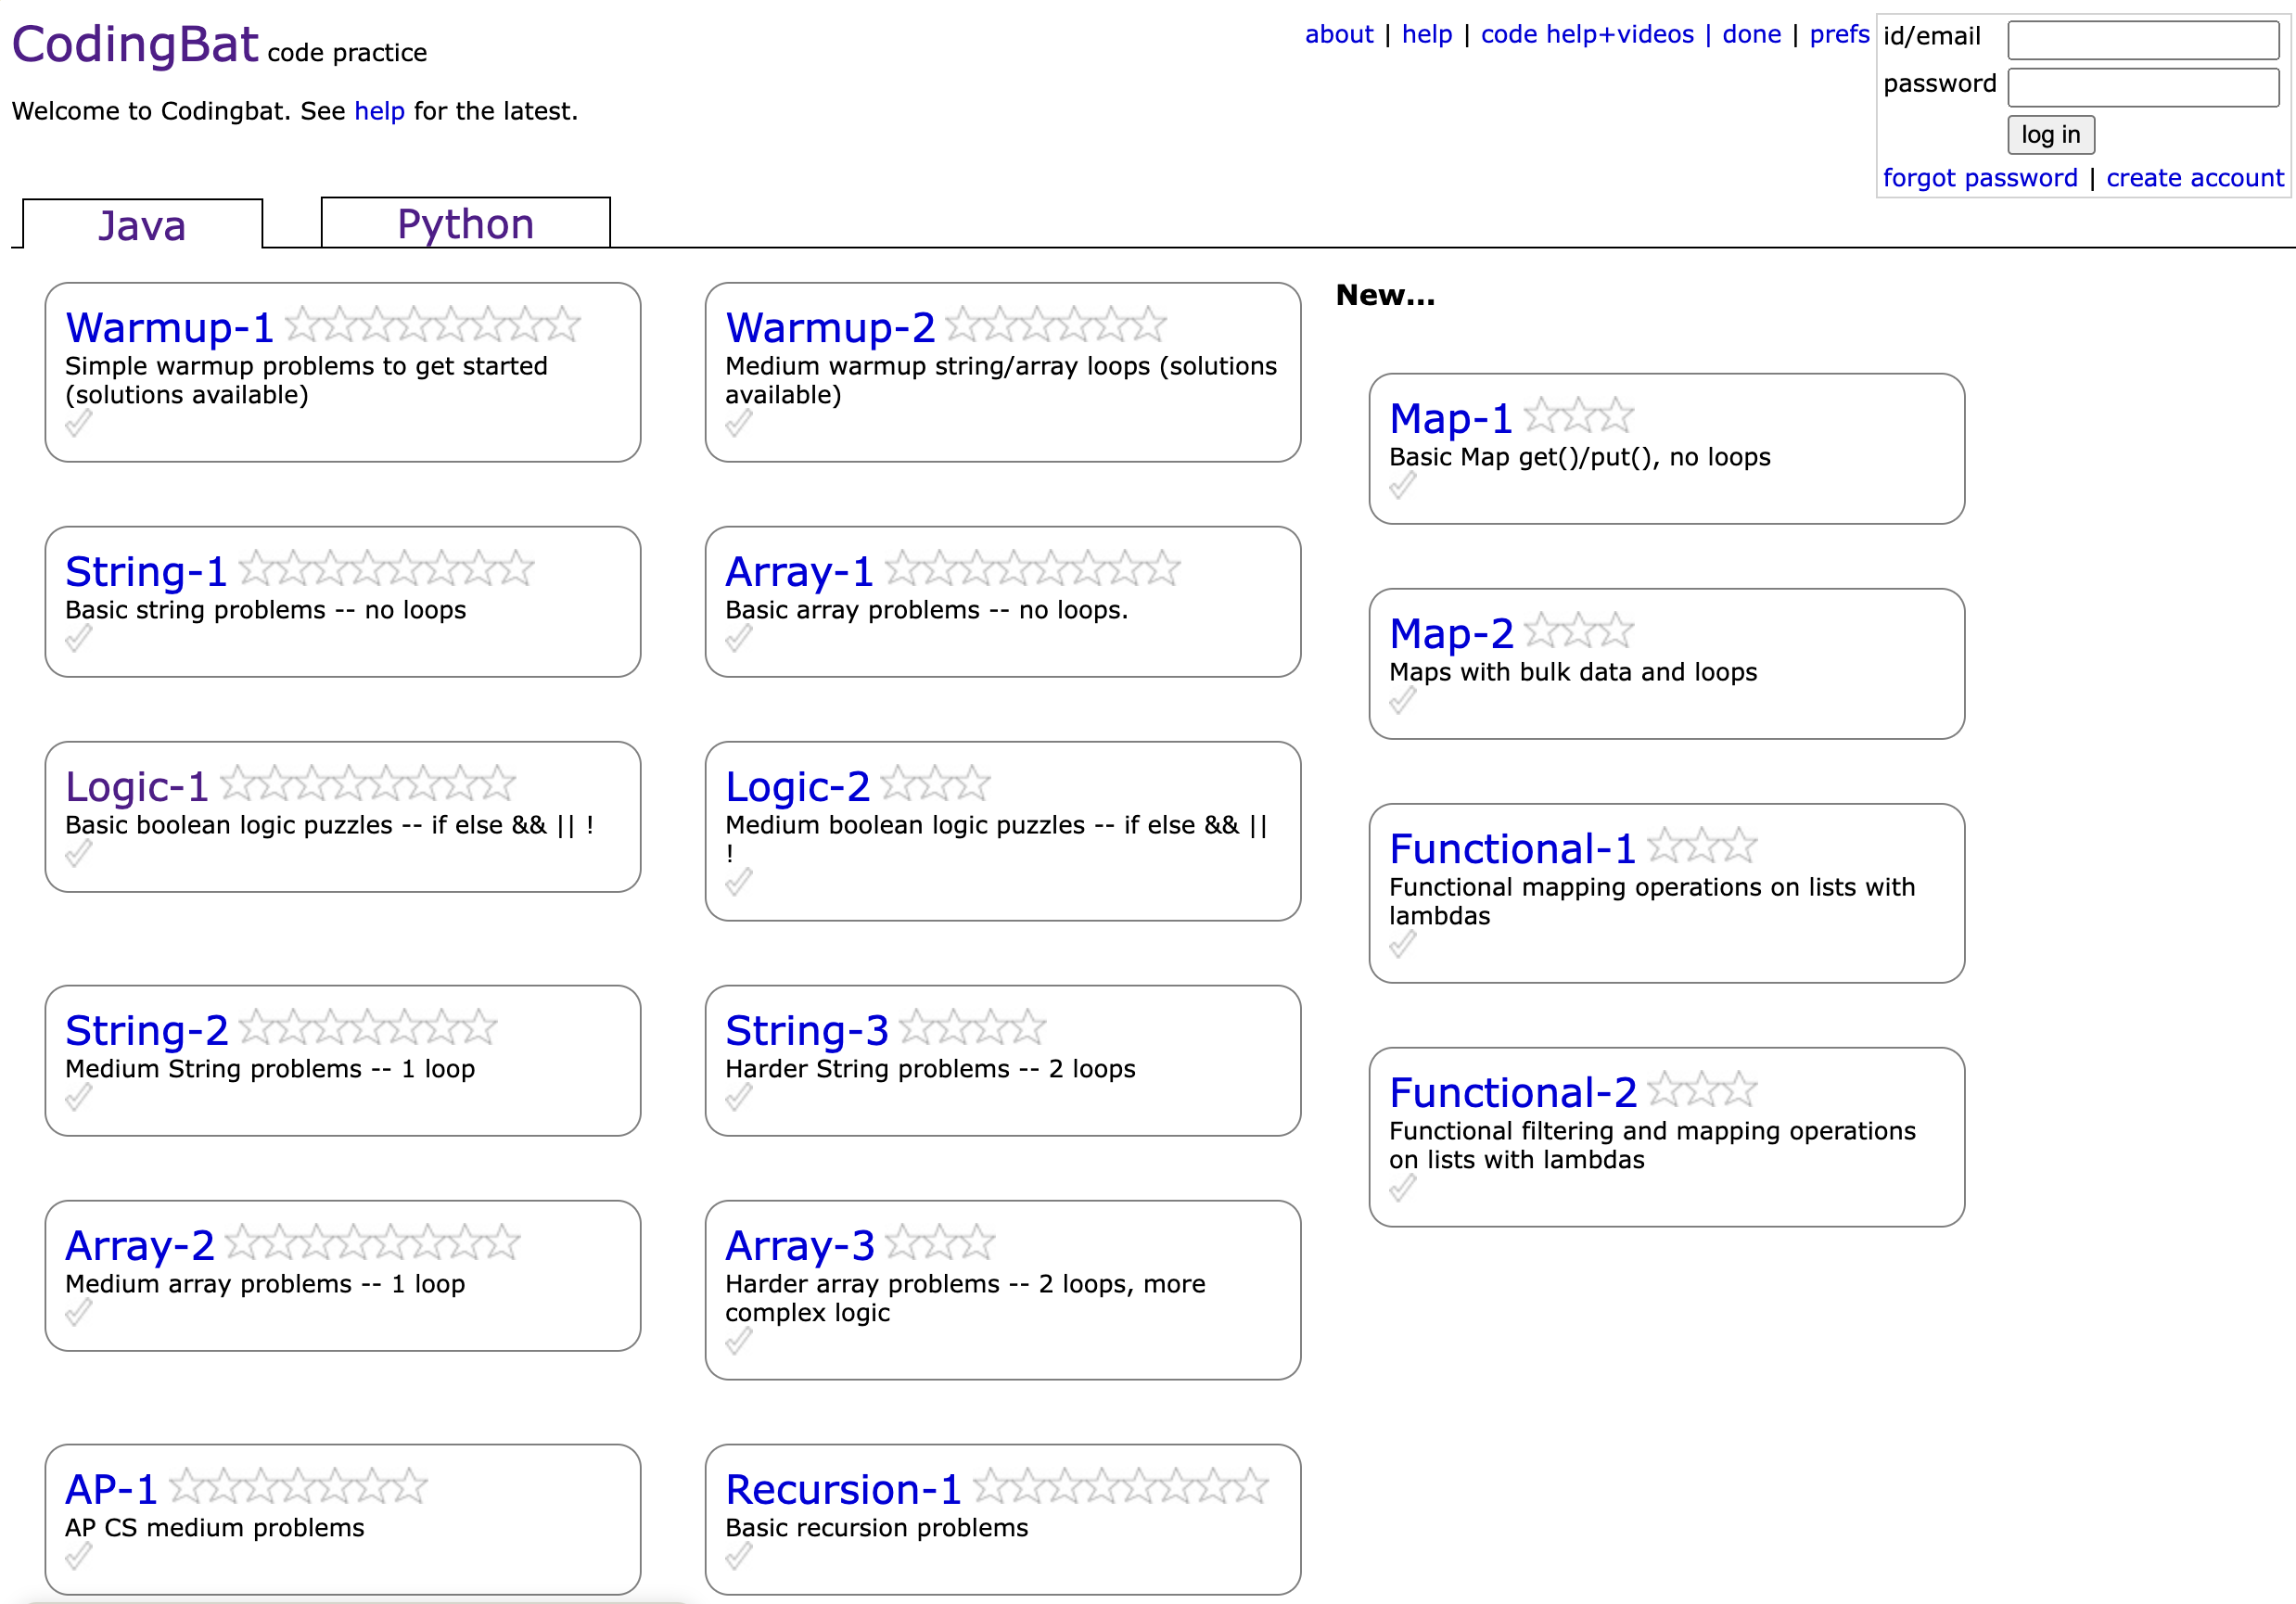
\includegraphics[width=.95\linewidth]{CodingBat0.png}
    \caption{
        Home page of CodingBat's coding exercises for Java.
    }
    \label{fig:first-page}
\end{figure}

\begin{figure}
    \centering
    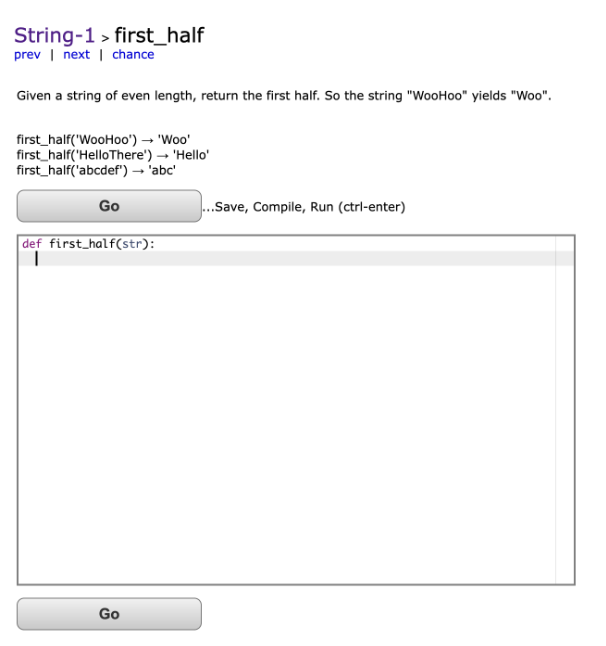
\includegraphics[width=.95\linewidth]{CodingBat1.png}
    \caption{
        One Python coding exercise in CodingBat.
    }
    \label{fig:first-page}
\end{figure}

\begin{figure}
    \centering
    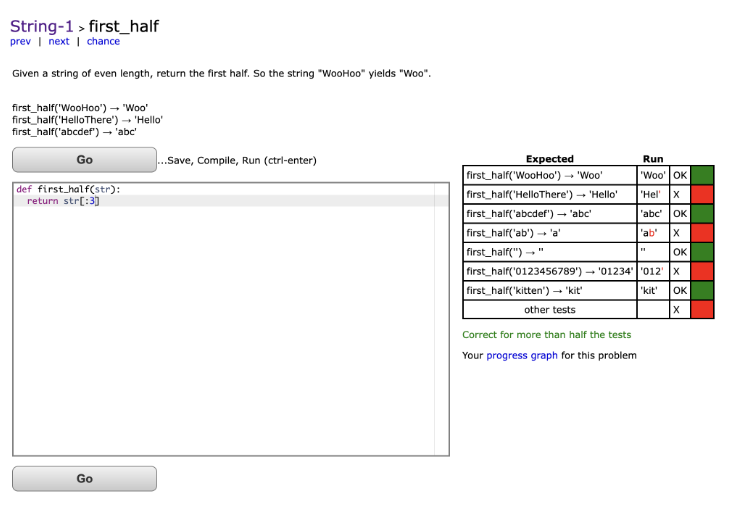
\includegraphics[width=.95\linewidth]{CodingBat2.png}
    \caption{
        Test cases for this function. Some test cases have failed, indicating an error in the code.
    }
    \label{fig:first-page}
\end{figure}

\begin{figure}
    \centering
    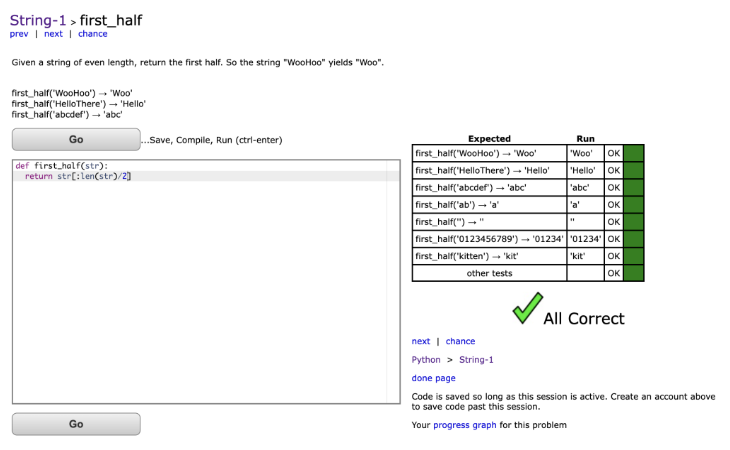
\includegraphics[width=.95\linewidth]{CodingBat3.png}
    \caption{
        All test cases have passed for this function.
    }
    \label{fig:first-page}
\end{figure}

My website will also have a similar overall structure, where the user is able to select a coding exercise, write their code, and test it. However, rather than only writing the code for the exercise, users will also be guided through writing their own test cases in addition to the pre-written ones. I will also create different levels of difficulty that users can progress through, as outlined in the Methods section. Ultimately, my goal is for users to find the experience engaging and continue to progress through the levels in order to ensure that they are getting the most out of it.

Two primary conferences relating to computer science education are the Special Interest Group on Computer Science Education (SIGCE) and International Computing Education Research (ICER). One paper from ICER’s 2023 conference, titled “Evaluating Beacons, the Role of Variables, Tracing, and Abstract Tracing for Teaching Novices to Understand Program Intent” discusses the importance of “program comprehension,” stating that “Skill in program comprehension is undoubtedly necessary to be a strong programmer. “Explain in Plain English” (EiPE) questions capture an important aspect of students’ program comprehension ability: the capacity to identify the overall purpose or intent of a piece of code [18]. This competency to explain code is not only useful on its own—it [has] also been consistently found to correlate with other programming skills, like code tracing and writing [9, 23, 25], suggesting that similar knowledge underlies all of these abilities” \cite{Teaching}. While this paper is not related to teaching students how to test their code, its discussion on methods to determine students’ comprehension of code provides an important set of guidelines for my website. For instance, rather than asking students to immediately dive into writing code and test cases to test it, it is helpful to have them answer certain questions in written English as a method of brainstorming. This will not only allow users to take a moment to understand the exercise and what the expected output for a given input should be. They will be able to think through their code and what test cases will allow them to ensure that their code is functioning as intended.

Another paper relevant to this project, titled “Test-Driven Learning: Intrinsic Integration of Testing into the CS/SE Curriculum,” discusses the concept of “test-driven learning (TDL),” which they define as “...an approach to teaching computer programming that involves introducing and exploring new concepts through automated unit tests. TDL offers the potential of teaching testing for free, of improving programmer comprehension and ability, and of improving software quality both in terms of design quality and reduced defect density.” The authors define the basic principles of TDL as: (1) “teach[ing] by example,” (2) “present[ing] examples with automated tests,” and (3) “start[ing] with tests.” They expand on these concepts; the first two points are connected, as showing students examples with automated tests is an instance of teaching by example: “Teaching by example has a double meaning in TDL. First TDL encourages instructors to teach by presenting examples with automated tests. Second, by holding tests in high regard and by writing good tests, instructors model good practices that contribute to a number of positive results. Students tend to emulate what they see modeled. So as testing becomes a habit formed by example and repetition, students may begin to see the benefits of developing software with tests and be motivated to write tests voluntarily.” The authors go on to expand on what it means to “start with tests,” as TDL can utilize a test-first or test-last approach: “The third aspect of TDL suggests a test-first approach. TDL could be applied in either a test-first or a test-last manner. With a test-last approach, a concept would be implemented, then a test would be written to demonstrate the concept’s use and behavior. With a test-first approach, the test would be written prior to implementing a concept. By writing a test before implementing the item under test, attention is focused on the item’s interface and observable behavior” \cite{Test-driven}. This paper provides useful guidelines for how to implement test-driven learning, which is certainly something that my project will utilize. Additionally, the test-first approach suggests that it may be helpful for my website to have users write some test cases before writing their code, while also letting them write additional ones later if needed. Doing so can allow users to take time to fully consider the instructions and expected behavior of the function or method before actually writing it.

Another paper discussing the test-first approach, titled “Rethinking Computer Science Education from a Test-first Perspective,” describes the importance of having students submit test cases along with their code for assignments. The author states that “...most undergraduate curricula focus on developing program application and synthesis skills (i.e., writing code), primarily acquired through hands-on activities.” However, many students don’t necessarily appreciate the complexity of an assignment from testing with no genuine strategy; according to the author, “Particularly during freshman and sophomore courses [for undergraduates], and occasionally much later, a student may believe that once the code she has written compiles successfully, the errors are gone. If the program runs correctly on the first few runs she tries, it must be correct. If there is a problem, maybe by switching a few lines around or tweaking the code by trial and error, it can be fixed.” This means that students often complete their coding assignments “without developing a broader view, which only reinforces approaches that will handicap their performance in more advanced courses.” Therefore, it is essential that students understand the importance of testing early on and work to develop those skills as they progress through computer programming courses. This paper focuses on developing “... a vision of a test-first-inspired educational strategy: systematically supporting test-first programming from the beginning to ensure students acquire the necessary comprehension and analysis skills needed to support effective programming” \cite{Test-first}. Just like the previous paper, this paper also demonstrates the effectiveness of having students write tests before writing code for the actual assignment, as it ensures that they take the time to understand the instructions.

\section{Methods}

Even in the early stages of the process of creating this website, it will be essential to talk to both students and professors. The purpose of these interviews with students will be to gain background information on their past and current experiences with computer programming and what they are looking for in a computer science education resource. Meanwhile, professors who teach classes that require coding in a variety of departments will be able to provide insight into how they teach students to test (if they do) and what they have found to be effective (or ineffective). Ideally, multiple interviews will be conducted with some participants in order to receive a continuous stream of feedback over the course of the development of the website.

I am currently planning on allowing users to select among a variety of exercises, with the difficulty level indicated for each. While I am not sure how I will determine the difficulty of each exercise, I will likely build on the method that CodingBat uses, which sorts exercises by the number of loops that they require (zero, one, or two) in addition to separating them by topic \cite{CodingBat}. As the main goal of my website is related to writing test cases, none of the exercises will require any knowledge beyond what is covered in the COMP 131 and COMP 181 courses. Users who are unfamiliar with certain concepts like arrays or lists and loops can start at some of the logic-based problems, which generally will only require the use of an if… else statement and operators (such as arithmetic, assignment, comparison, and logical operators). The earlier exercises will guide users through the entire process of writing the function or method if they need the assistance, and each time a new concept is introduced, users will also be able to receive guidance if it is unfamiliar to them. In order for users to have a clear understanding of all of the available exercises, the concepts that they introduce and/or require knowledge of, and their level of difficulty, there will be a syllabus that outlines all of this information. It is fully up to the users to select the exercises that they feel are appropriate for them given their background knowledge. For users who have already mastered all of the concepts, there will be a “challenge section” that does not present any new information, but contains more challenging exercises that may require them to write significantly longer functions or methods, as well as several helper functions or methods. Similar to CodingBat, users will be able to keep track of the exercises that they have completed, and completing a certain number of exercises covering different concepts will earn users a certain type of badge.

For each exercise, users will first be presented with the instructions and given space to write pseudocode and write some thoughts down. For some of the more introductory exercises, there will be specific questions which users will have the opportunity to answer, designed to help them comprehend the instructions and “overall purpose” of the exercise. These will be modeled after the “Explain in Plain English” (EiPE) questions discussed in the ““Evaluating Beacons, the Role of Variables, Tracing, and Abstract Tracing for Teaching Novices to Understand Program Intent” paper \cite{Teaching}. Some questions will be designed to simply have users spend some time thinking about the exercise, while others will have correct answers. For example, a question might ask how many arguments the function or method has. For questions like these, users will be able to see the correct answer after responding. I am still unsure of whether I would like to have users write several test cases before beginning to code for the exercise (the test-first approach), or whether that will be left up to them to decide. Given the benefits of this approach outlined in the two papers \cite{Test-driven} \cite{Test-first}, I believe that asking users to write at least a few test cases will allow them to appreciate the scope of each exercise. Even though some simple exercises might not allow users to develop a “broader view" \cite{Test-first}, it will likely be good practice for the more challenging exercises. Therefore, I will likely have users write a few test cases before beginning to code. When users write test cases, they will be able to choose the inputs and make note of the expected output. After this has been completed, users will be able to write the function or method and additional tests (or all of the tests, if I decide to instead use a test-last approach). In addition to the user’s written test cases, each exercise will be accompanied by some pre-written test cases, which may be auto-generated so that they are different for each user. Having these auto-generated test cases can ensure that they are truly randomized, but it may leave out several important edge cases. Therefore, I will likely work to ensure that the pre-written test cases contain these essential edge cases, while additional test cases will be generated. The user’s code will also be checked using fuzz testing. If there are any issues with the user’s code, (if any of the tests result in something other than the expected output) the user will be able to go back, edit their code, and run the tests again. If the user simply expects an incorrect output from their own test cases but their code works as intended, all of the pre-written and generated test cases should pass. All coding exercises will have solutions. Ideally, I would like to include several different ways of writing the function or method, which may differ in their length and approach.

In summary, the user inputs will consist of written English sentences which will not be “checked” in any way by the website, a few questions with correct answers (either a numerical value or one-word answer) which will be checked for accuracy by comparing them to the correct numerical value or string, code which will be checked with test cases, and the user generated test cases themselves. There likely won’t be any “check” for whether the user’s test cases and the noted expected outputs make sense; if they fail but all of the pre-written and website-generated test cases pass, then the user will be asked to check their inputs and noted expected output.

\section{Evaluation Metrics}

In order to evaluate the effectiveness of my project, it is essential to conduct user research. Rather than using a survey, I will be conducting interviews with students and professors to gain insight into different individuals' experiences with learning and/or teaching computer programming. For my projects, interviews will be a preferable method of user testing because they allow for a more individualized approach. In the responses from the survey outlined in my tutorial report, there were not many responses to the open-ended questions that allowed users to expand on their thoughts about the two agree/disagree statements or what resources they have found helpful when facing challenges. With interviews, it will be easier to ask participants to expand on a thought or experience. Additionally, the questions can be modified depending on the background that each participant has with computer programming. For students, I will utilize some of the same questions as those included in the survey discussed in my tutorial report \cite{Tutorial}, such as:
\begin{itemize}
    \item Were there any computer science classes offered at your high school? If so, did you take one or more computer science classes in high school?
    \item{Have you taken and/or are you currently taking any computer science courses at Oxy? If so, which computer science course(s) have you taken and/or are you currently taking?}
    \item{For non-seniors: Do you plan on taking any (additional) computer science courses in your remaining time at Oxy?}
    \item{Have you ever had to write code in a non-computer science course at Oxy? If so, which one(s)?}
    \item{If you have taken and/or are currently taking any course that requires coding (including non-computer science courses), what resources have you utilized when experiencing challenges?}
    \item{To what degree do you agree or disagree with the following statement? It is important for everyone to have some basic coding knowledge, regardless of the field that they choose to pursue.}
    \item{To what degree do you agree or disagree with the following statement? I would like to learn some foundational coding skills OR I would like to continue building on my existing coding skills in the future.}
\end{itemize}
However, as I progress with different aspects of creating the website, I will ensure to continuously seek student feedback by having them share their thoughts and experiences when using the website. Some questions that I could ask include:
\begin{itemize}
    \item{How do you find the difficulty level of the exercises given your level of experience with coding?}
    \item{Which aspects (if any) of the instruction are effective? Which aspects (if any) are not? (This is specifically related to the teaching methods designed to teach users how to effectively test code.)}
    \item{Do you find the test-first approach to be effective? Do you find the ““Explain in Plain English” (EiPE) style-questions effective? Why or why not?}
\end{itemize}

It will also be essential to gain insight into computer science education from professors, both in the Computer Science department and professors in other departments who teach courses requiring computer programming, such as Physics, Economics, Media Arts and Culture, and Cognitive Science. These professors can provide valuable information regarding their experiences teaching students with a wide variety of past coding experience, their observations with the areas of computer literacy and/or programming that students most struggle with, and what resources have worked well for students (as well as which ones haven’t and for what reasons). Ideally, I would like to speak to professors who have taught introductory computer science courses (COMP 131: Fundamentals of Computer Science and COMP 181: Advanced Programming), as well as professors in the other four listed departments who teach courses such as Experimental Game Making (Media Arts and Culture), Computational Neuroscience (Cognitive Science), and Simulations in Physics and Advanced Laboratory (Physics). I will ask them to provide similar feedback to the last two questions listed above for students. Additionally, I will ask them to discuss their approach to teaching students about testing code and what strategies and/or teaching techniques they have found to be effective and ineffective. User testing will likely be one of the most important and challenging aspects of my project, so I will ensure that I devote a sufficient amount of time to gathering this valuable feedback and making iterations to my project as necessary.

\section{Timeline}

Below is a list of what I would like to work on for every two week period.

\begin{itemize}
    \item{May 6 + May 13: Continue conducting research on the process of creating a website using JavaScript and learning more about how to write fuzz tests.}
    \item{May 20 + May 27: Work on creating a website using JavaScript that accomplishes some simple task and allows for the user to interact in some way, such as a tip calculator where the user indicates the bill amount and desired tip percentage or a to-do list maker where a user can enter tasks and mark them as completed. Work on writing fuzz tests by rewriting unit tests.}
    \item{June 3 + June 10: Create a general outline of the website, including some possible exercises and the different levels of difficulty that users will be able to progress through, with particular emphasis on how testing will be taught over these levels.}
    \item{June 17 + June 24: Continue practicing JavaScript and improve on the projects made during the weeks of May 20 and May 27.}
    \item{July 1 + July 8: Continue working on anything from the past weeks that is unfinished or I would benefit from spending more time on.}
    \item{July 15 + July 22: Plan out interview questions for both students and professors, with particular emphasis on gaining insight into how they have been taught about testing (for students) or have taught testing (for professors) and understanding students’ and professors’ goals and motivations in different courses.}
    \item{July 29 + August 5: Begin writing actual code for the website and document the process.}
    \item{August 12 + August 19: Continue building the website and documenting the process, with a particular emphasis on writing the website-generated test cases.}
    \item{August 26 + September 2: Send out emails to students and professors for interviews and finalize interview questions. Then, set up an interview schedule over the course of the semester, first focusing on gaining background information about the participants and asking about their first thoughts on the website’s design and later on getting their feedback on the website’s progression.}
    \item{September 9 + September 16: Continue writing the code and documentation for the website and seek out assistance for any trouble areas.}
    \item{September 23 + September 30: Finish writing all of the exercises and information on testing for the website. Work on writing the paper using this proposal and make changes as necessary.}
    \item{October 7 + October 14: Finish writing all of the test cases for the website-generated test cases for each exercise and continue working on the paper.}
    \item{October 21 + October 28: Continue working on my project (both the code and paper) and make the necessary changes from the feedback gathered from interviews.}
    \item{November 4 + November 11: Work on creating my poster for the poster presentation and continue finalizing my project.}
    \item{November 18 + November 25: Prepare for the poster presentation and finalize my project (the code).}
    \item{December 2 + December 9: Finalize my paper and make any final changes to the website based on faculty feedback from the poster presentation.}
\end{itemize}

\printbibliography

\end{document}